%% abtex2-modelo-trabalho-academico.tex, v-1.9.2 laurocesar
%% Copyright 2012-2014 by abnTeX2 group at http://abntex2.googlecode.com/ 
%%
%% This work may be distributed and/or modified under the
%% conditions of the LaTeX Project Public License, either version 1.3
%% of this license or (at your option) any later version.
%% The latest version of this license is in
%%   http://www.latex-project.org/lppl.txt
%% and version 1.3 or later is part of all distributions of LaTeX
%% version 2005/12/01 or later.
%%
%% This work has the LPPL maintenance status `maintained'.
%% 
%% The Current Maintainer of this work is the abnTeX2 team, led
%% by Lauro César Araujo. Further information are available on 
%% http://abntex2.googlecode.com/
%%
%% This work consists of the files abntex2-modelo-trabalho-academico.tex,
%% abntex2-modelo-include-comandos and abntex2-modelo-references.bib
%%

% ------------------------------------------------------------------------
% ------------------------------------------------------------------------
% abnTeX2: Modelo de Trabalho Academico (tese de doutorado, dissertacao de
% mestrado e trabalhos monograficos em geral) em conformidade com 
% ABNT NBR 14724:2011: Informacao e documentacao - Trabalhos academicos -
% Apresentacao
% ------------------------------------------------------------------------
% ------------------------------------------------------------------------

\documentclass[
	% -- opções da classe memoir --
	12pt,				% tamanho da fonte
	openright,			% capítulos começam em pág ímpar (insere página vazia caso preciso)
	oneside,			% para impressão em verso e anverso. Oposto a oneside
	a4paper,			% tamanho do papel. 
	% -- opções da classe abntex2 --
	%chapter=TITLE,		% títulos de capítulos convertidos em letras maiúsculas
	%section=TITLE,		% títulos de seções convertidos em letras maiúsculas
	%subsection=TITLE,	% títulos de subseções convertidos em letras maiúsculas
	%subsubsection=TITLE,% títulos de subsubseções convertidos em letras maiúsculas
	% -- opções do pacote babel --
	english,			% idioma adicional para hifenização
	french,				% idioma adicional para hifenização
	spanish,			% idioma adicional para hifenização
	brazil				% o último idioma é o principal do documento
	]{abntex2}

% ---
% Pacotes básicos 
% ---
\usepackage{times}			% Usa a fonte Times new Romam			
\usepackage[T1]{fontenc}		% Selecao de codigos de fonte.
\usepackage[utf8]{inputenc}		% Codificacao do documento (conversão automática dos acentos)
\usepackage{lastpage}			% Usado pela Ficha catalográfica
\usepackage{indentfirst}		% Indenta o primeiro parágrafo de cada seção.
\usepackage{color}				% Controle das cores
\usepackage{graphicx}			% Inclusão de gráficos
\usepackage{microtype} 			% para melhorias de justificação
\usepackage{lipsum}				% para geração de dummy text
\usepackage[alf]{abntex2cite}	% Citações padrão ABNT
\usepackage{scalefnt}
\usepackage[portuguese, ruled, linesnumbered]{algorithm2e}

% ---
% Informações de dados para CAPA e FOLHA DE ROSTO
% ---
\titulo{Modelo canônico abnt latex UEPG}
\autor{Nome do autor}
\local{\textbf{PONTA GROSSA}}
\data{\textbf{2018}}
\orientador{Seu orientador}
\coorientador{Seu coorientador}
\instituicao{%
  UNIVERSIDADE ESTADUAL DE PONTA GROSSA
  \par
  SETOR DE CIÊNCIAS AGRÁRIAS E DE TECNOLOGIA
  \par
  PROGRAMA DE PÓS-GRADUAÇÃO EM COMPUTAÇÃO APLICADA}
\tipotrabalho{Dissertação (Mestrado)}
% O preambulo deve conter o tipo do trabalho, o objetivo, 
% o nome da instituição e a área de concentração 
\preambulo{Trabalho de Conclusão de Curso apresentado para a obtenção do título de Mestre em Computação Aplicada pela Universidade Estadual de Ponta Grossa - UEPG}
% ---


% ---
% Configurações de aparência do PDF final

% alterando o aspecto da cor azul
\definecolor{blue}{RGB}{41,5,195}

% informações do PDF
\makeatletter
\hypersetup{
     	%pagebackref=true,
		pdftitle={\@title}, 
		pdfauthor={\@author},
    	pdfsubject={\imprimirpreambulo},
	    pdfcreator={LaTeX with abnTeX2},
		pdfkeywords={abnt}{latex}{abntex}{abntex2}{trabalho acadêmico}, 
		colorlinks=true,       		% false: boxed links; true: colored links
    	linkcolor=blue,          	% color of internal links
    	citecolor=blue,        		% color of links to bibliography
    	filecolor=magenta,      		% color of file links
		urlcolor=blue,
		bookmarksdepth=4
}
\makeatother
% --- 

% --- 
% Espaçamentos entre linhas e parágrafos 
% --- 

% O tamanho do parágrafo é dado por:
\setlength{\parindent}{1.3cm}

% Controle do espaçamento entre um parágrafo e outro:
\setlength{\parskip}{0.2cm}  % tente também \onelineskip

% ---
% compila o indice
% ---
\makeindex
% ---

% ---
%\makeglossaries
% ---

% ----
% Início do documento
% ----
\begin{document}

% Retira espaço extra obsoleto entre as frases.
\frenchspacing 
\imprimircapa
\imprimirfolhaderosto*

% ---
% Inserir a ficha bibliografica
% ---

% Isto é um exemplo de Ficha Catalográfica, ou ``Dados internacionais de
% catalogação-na-publicação''. Você pode utilizar este modelo como referência. 
% Porém, provavelmente a biblioteca da sua universidade lhe fornecerá um PDF
% com a ficha catalográfica definitiva após a defesa do trabalho. Quando estiver
% com o documento, salve-o como PDF no diretório do seu projeto e substitua todo
% o conteúdo de implementação deste arquivo pelo comando abaixo:
%
% \begin{fichacatalografica}
%     \includepdf{fig_ficha_catalografica.pdf}
% \end{fichacatalografica}

\begin{fichacatalografica}
	\vspace*{\fill}					% Posição vertical
	\hrule							% Linha horizontal
	\begin{center}					% Minipage Centralizado
	\begin{minipage}[c]{12.5cm}		% Largura
	
	\imprimirautor
	
	\hspace{0.5cm} \imprimirtitulo  / \imprimirautor. --
	\imprimirlocal, \imprimirdata-
	
	\hspace{0.5cm} \pageref{LastPage} p. : il. (algumas color.) ; 30 cm.\\
	
	\hspace{0.5cm} \imprimirorientadorRotulo~\imprimirorientador\\
	
	\hspace{0.5cm}
	\parbox[t]{\textwidth}{\imprimirtipotrabalho~--~\imprimirinstituicao,
	\imprimirdata.}\\
	
	\hspace{0.5cm}
		1. Palavra-chave1.
		2. Palavra-chave2.
		I. Orientador.
		II. Universidade xxx.
		III. Faculdade de xxx.
		IV. Título\\ 			
	
	\hspace{8.75cm} CDU 02:141:005.7\\
	
	\end{minipage}
	\end{center}
	\hrule
\end{fichacatalografica}
% ---
% ---
% Inserir errata
% ---
\begin{errata}
Elemento opcional da \citeonline[4.2.1.2]{NBR14724:2011}. Exemplo:

\vspace{\onelineskip}

FERRIGNO, C. R. A. \textbf{Tratamento de neoplasias ósseas apendiculares com
reimplantação de enxerto ósseo autólogo autoclavado associado ao plasma
rico em plaquetas}: estudo crítico na cirurgia de preservação de membro em
cães. 2011. 128 f. Tese (Livre-Docência) - Faculdade de Medicina Veterinária e
Zootecnia, Universidade de São Paulo, São Paulo, 2011.

\begin{table}[htb]
\center
\footnotesize
\begin{tabular}{|p{1.4cm}|p{1cm}|p{3cm}|p{3cm}|}
  \hline
   \textbf{Folha} & \textbf{Linha}  & \textbf{Onde se lê}  & \textbf{Leia-se}  \\
    \hline
    1 & 10 & auto-conclavo & autoconclavo\\
   \hline
\end{tabular}
\end{table}

\end{errata}
% ---

% ---
% Inserir folha de aprovação
% ---

% Isto é um exemplo de Folha de aprovação, elemento obrigatório da NBR
% 14724/2011 (seção 4.2.1.3). Você pode utilizar este modelo até a aprovação
% do trabalho. Após isso, substitua todo o conteúdo deste arquivo por uma
% imagem da página assinada pela banca com o comando abaixo:
%
% \includepdf{folhadeaprovacao_final.pdf}

\begin{folhadeaprovacao}

  \begin{center}
    {\ABNTEXchapterfont\large\imprimirautor}

    \vspace*{\fill}\vspace*{\fill}
    \begin{center}
      \ABNTEXchapterfont\bfseries\Large\imprimirtitulo
    \end{center}
    \vspace*{\fill}
    
    \hspace{.45\textwidth}
    \begin{minipage}{.5\textwidth}
        \imprimirpreambulo
    \end{minipage}%
    \vspace*{\fill}
   \end{center}
        
   Trabalho aprovado. \imprimirlocal, 24 de novembro de 2012:

   \assinatura{\textbf{\imprimirorientador} \\ Orientador} 
   \assinatura{\textbf{Professor} \\ Convidado 1}
   \assinatura{\textbf{Professor} \\ Convidado 2}
   %\assinatura{\textbf{Professor} \\ Convidado 3}
   %\assinatura{\textbf{Professor} \\ Convidado 4}
      
   \begin{center}
    \vspace*{0.5cm}
    {\large\imprimirlocal}
    \par
    {\large\imprimirdata}
    \vspace*{1cm}
  \end{center}
  
\end{folhadeaprovacao}
% ---
\

\vfill

\begin{flushright}
\hfill \textit{Dedico este trabalho aos meus queridos pais,\\ que por amor fizeram de tudo por mim. }
\end{flushright}

\vspace*{1cm}

\clearpage
\chapter*{Agradecimentos}
À Deus, que esteve presente em todos os momentos, me guiou com sua luz divina, ouviu minhas preces e me fortaleceu. A Ti, meu Deus, toda honra e toda glória eternamente.
% ---
% Epígrafe
% ---
\begin{epigrafe}
    \vspace*{\fill}
	\begin{flushright}
		\textit{``Não vos amoldeis às estruturas deste mundo, \\
		mas transformai-vos pela renovação da mente, \\
		a fim de distinguir qual é a vontade de Deus: \\
		o que é bom, o que Lhe é agradável, o que é perfeito.\\
		(Bíblia Sagrada, Romanos 12, 2)}
	\end{flushright}
\end{epigrafe}
% ---
\begin{resumo}

{\noindent A Qualidade de Vida (QV) é definida pela Organização Mundial de Saúde (OMS) como algo subjetivo e de natureza multidimensional, visto que vários fatores a influenciam. Estudos recentes demonstram que a condição bucal pode atuar como um fator modificador para a QV de indivíduos portadores de doenças crônicas. Objetivo: Avaliar o impacto da saúde bucal sobre a qualidade de vida de pacientes com Doença Renal Crônica (DRC) em Hemodiálise (HD). Métodos: Trata-se de um estudo caso controle de caráter observacional e transversal, com aplicação de questionários estruturados para 100 pacientes com DRC em hemodiálise (Grupo DRC) pareados com 100 pacientes controles (Grupo Controle). Os dados demográficos e de escolaridade foram obtidos em formulário elaborado especificamente para a pesquisa. A classificação da condição socioeconômica seguiu os critérios da Associação Brasileira de Empresas de Pesquisas. A qualidade de vida, bem como, o impacto da saúde bucal sobre a QV foi avaliado através dos seguintes questionários respectivamente: 1) “\textit{The Short Form Health Survey} (SF-36)” e 2) “\textit{Oral Health Impact Profile-14} (OHIP-14)”. Resultados: A média total do OHIP-14 para o grupo controle foi de 6,06 ($\pm$ 7,44) e de 4,67 ($\pm$ 6,52) para o grupo DRC. Ao comparar os valores internos do OHIP-14 entre os grupos controle e DRC, não foi observado diferença estatisticamente significativa entre os grupos. Em relação a qualidade de vida geral avaliada pelo SF-36, o grupo DRC obteve os piores scores para os domínios “capacidade funcional” e “limitação por aspectos físicos”. Em relação a QV geral no grupo controle, este grupo apresentou pior pontuação no domínio de “limitação por aspectos emocionais”. Foi observada correlação negativa fraca entre as características odontológicas e os valores obtidos do questionário OHIP-14. Conclusões: Os pacientes com DRC em HD apresentaram um baixo impacto da saúde bucal sobre a qualidade de vida. Além disso, pacientes DRC têm uma pior Qualidade de Vida Relacionada a Saúde (QVRS) nos domínios internos “capacidade funcional” e “limitação por aspectos físicos”, sendo que as mulheres e idosos manifestam mais a influência da doença. No sentido de que o tratamento aos DRC não deve visar somente a sobrevivência, mas também maximizar a reabilitação e a QV, sugere-se que uma atenção integral aliada a uma equipe multidisciplinar possa contribuir para o sucesso no tratamento da doença base e uma melhoria na qualidade de vida geral destes indivíduos.\\

}
{\noindent \textbf{Palavras-chave:}  Qualidade de vida. Impacto da saúde bucal. Doença renal crônica.}

\end{resumo}

% ---
% inserir lista de ilustrações
% ---
\pdfbookmark[0]{\listfigurename}{lof}
\listoffigures*
\cleardoublepage
% ---

% ---
% inserir lista de tabelas
% ---
\pdfbookmark[0]{\listtablename}{lot}
\listoftables*
\cleardoublepage
% ---

% ---
% inserir lista de abreviaturas e siglas
% ---
\begin{siglas}
  \item[ABNT] Associação Brasileira de Normas Técnicas
  \item[abnTeX] ABsurdas Normas para TeX
\end{siglas}
% ---

% ---
% inserir lista de símbolos
% ---
\begin{simbolos}
  \item[$ \Gamma $] Letra grega Gama
  \item[$ \Lambda $] Lambda
  \item[$ \zeta $] Letra grega minúscula zeta
  \item[$ \in $] Pertence
\end{simbolos}
% ---

% ---
% inserir o sumario
% ---
\pdfbookmark[0]{\contentsname}{toc}
\tableofcontents*
\cleardoublepage
% ---

% ----------------------------------------------------------
% ELEMENTOS TEXTUAIS
% ----------------------------------------------------------
\textual

\chapter[INTRODUÇÃO]{INTRODUÇÃO}


\chapter[OBJETIVO]{OBJETIVO}
\chapter[REVISÃO]{REVISÃO}
\chapter{MATERIAIS E MÉTODOS}

\section{CARACTERÍSTICAS GERAIS}
texto
\chapter[RESULTADO]{RESULTADO}
\chapter[DISCURSSÃO]{DISCURSSÃO}
\chapter[CONCLUSÃO]{CONCLUSÃO}
\bibliography{abntex2-modelo-references}
%---------------------
%Glossário
%---------------------
%\newglossaryentry{ambiguidade}{
	name=Ambiguidade,
	description={possibilidade de interpretação dúbia de uma palavra ou frase}
}

\newglossaryentry{braile}{
	name=Braile,
	description={sistema de escrita para cegos. São signos desenhados em relevo para serem lidos com a ponta dos dedos}
}

\newglossaryentry{borboleta}{
	name=Borboleta,
	description={inseto voador, que possui dois pares de asas. São todos os insetos alados da família dos lepidópteros diurnos. São encontrada na natureza com diversas cores e tamanho}
}

\newglossaryentry{coerencia}{
	name=Coerência,
	description={qualidade subjacente a um texto, que lhe permite ter sentido}
}

\newglossaryentry{dialetos}{
	name=Dialetos,
	description={variedades regionais ou sociais de uma língua}
}

\newglossaryentry{elipse}{
	name=Elipse,
	description={omissão de termos da oração}
}

\newglossaryentry{locucao-adjetiva}{
	name=Locução Adjetiva,
	description={duas ou mais palavras que equivalem a um adjetivo}
}

\newglossaryentry{modificadores}{
	name=Modificadores,
	description={adjetivos}
}

\newglossaryentry{paronimos}{
	name=Parônimos,
	description={palavras que possuem sons parecidos. Exemplo: emigrar / imigrar}
}

\newglossaryentry{sintese}{
	name=Síntese,
	description={exposição resumida, em que se usa um mínimo de palavras}
}

%\setglossarystyle{tree}
%\cleardoublepage
%\phantomsection
%\addcontentsline{toc}{chapter}{\glossaryname}
%\printglossaries
%--------------------

\appendix
%Apendice A -----------------------------------------------------------------------------------------------------
\chapter{Resultados dos Tempos de Execução}

\section{Ferramenta \textit{Fast Weka}}
A ferramenta \textit{Fast Weka} tem também como objetivo ser de fácil utilização a todos aqueles que necessitam de uma ferramenta de mineração de dados, ou que já utilizam a ferramenta Weka, mas que tem suas tarefas de mineração demandando de um alto tempo de execução e buscam melhor desempenho.

Assim, como principal e única mudança visual realizada na ferramenta Weka, ocorreu a criação de uma tela inicial de configuração, onde são definidas as configurações de execução concorrente ou paralela, conforme a figura \ref{fig:telainicial}.

\begin{figure}[h!]

\centering
\caption{Tela Inicial \textit{Fast Weka}}

\includegraphics[width=0.8\textwidth,natwidth=610,natheight=642]{wekap2p.png}

\text{\footnotesize Fonte: O autor}
\label{fig:telainicial}
\end{figure}

Está tela é carregada toda vez que o programa é iniciado com a execução do arquivo fastweka.jar, ou por meio da linha de comando:
\begin{Verbatim}[frame=single]
java -cp fastweka.jar weka.gui.GUIChooser
\end{Verbatim}

Por padrão, a opção \textit{Application Running Locally} está pré-selecionada, que é utilizada quando deseja-se uma execução concorrente na maquina em questão (modo multi-\textit{threads}), o campo \textit{Number of Concurrent Requests} inicializa com o número máximo de núcleos do computador, considerando os núcleos reais e virtuais, podendo receber um valor entre um e o número máximo de núcleos do computador, o qual vai delimitar o número de execuções concorrente (\textit{Threads}).

A segunda opção disponível é \textit{Application Running on the P2P Network}, quando deseja-se realizar uma execução de modo paralelo com redes P2P, com está opção selecionada o campo citado acima é desabilitado e são habilitados os campos: \textit{IP/Name Rendezvous}, \textit{IP/Name Relay}, os dois campos \textit{Port} e também o campo \textit{Number of Peers}.

O campo \textit{Number of Peers} é responsável por definir o número de pares da rede P2P, os quais devem estar disponíveis para a execução das tarefas de mineração de dados, o mesmo aceita valores entre 2 até N.  Os outros campos supracitados, identificam os endereços de IP/Nome e Porta, do \textit{Rendezvous} e \textit{Relay} que são responsáveis pela concentração dos anúncios e informações de roteamento, respectivamente, podendo os dois estarem definidos no mesmo endereço.

Para iniciar a aplicação em modo \textit{Rendezvous}/\textit{Relay} deve-se utilizar o fastweka.jar por meio da linha de comando:
\begin{Verbatim}[frame=single]
java -cp fastweka.jar weka.p2p.RunRendezvous
\end{Verbatim}

Com os pares da rede P2P, também deve ser usado o fastweka.jar, porém com a linha de comando:
\begin{Verbatim}[frame=single]
java -cp fastweka.jar weka.p2p.StartPeer
\end{Verbatim}

Para que os pares encontrem o endereço do \textit{Rendezvous} e \textit{Relay}, e necessário que existam os arquivos: relay.txt e seeds.txt, no mesmo diretório onde encontra-se o arquivo fastweka.jar, contendo a informação do IP/Nome e Porta (tcp://IP/Nome:Porta), onde estão localizados os mesmo, exemplo:
\begin{Verbatim}[frame=single]
tcp://localhost:9701
\end{Verbatim}
\chapter*{\textbf{ANEXOS}}

\centering
ANEXO I
\begin{figure}[h!]
\centering
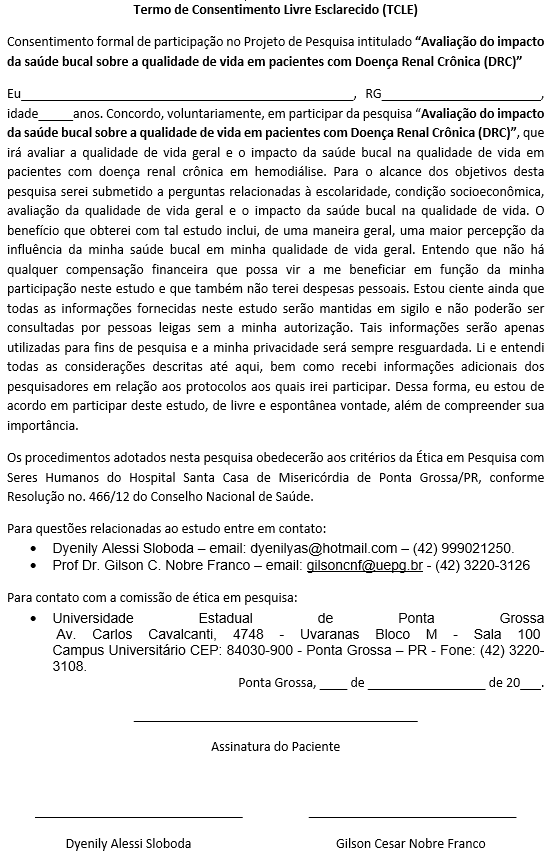
\includegraphics[width=0.62\textwidth]{imagens/anexo1}
\captionsetup{labelformat=empty}
\end{figure}
%---------------------------------------------------------------------
% INDICE REMISSIVO
%---------------------------------------------------------------------
\phantompart
\printindex
%---------------------------------------------------------------------


\end{document}